\documentclass[11pt,fleqn]{article}

\setlength {\topmargin} {-.15in}
\setlength {\textheight} {8.6in}

\usepackage{amsmath}
\usepackage{amssymb}
\usepackage{color}
\usepackage{tikz}
\usetikzlibrary{automata,positioning,arrows}
\usepackage{diagbox}
\usepackage{stackrel}
\begin{document}


\textbf{Exercise 1.3.48:} Two stacks with a deque. Implement two stacks with a single deque so that each
operation takes a constant number of deque operations (see Exercise 1.3.33)..\\

\textbf{Background information:} Recall a deque(or double-ended queue) is like a stack or queue but supports adding and removing items at both ends.\\

It consists of a few operations:\\ $Dequeue, isEmpty, size(), pushRight(Item item), popLeft, pushLeft(Item item), etc$ \\

\textbf{Solution:} So essentially, 2 stacks w/ one representing pushes/pops on RHS while the other stack is for pushes/[p[s on LHS.


\begin{center}
	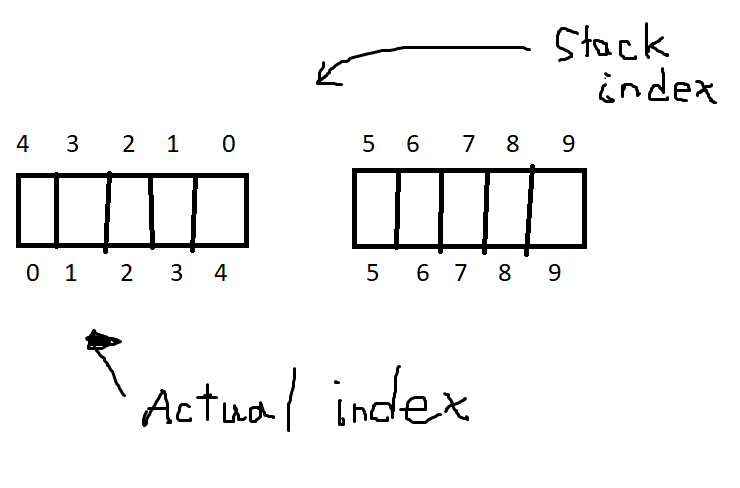
\includegraphics[scale = 1]{1.3.48.png}
	\end{center}
	
\newpage

Pseudocode below:

\begin{center}
	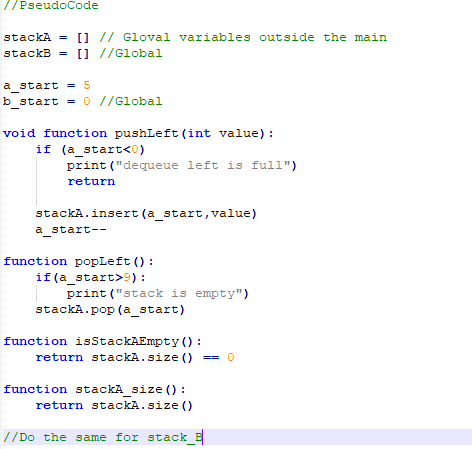
\includegraphics[scale = 1]{1.3.48-2.png}
	\end{center}

\end{document}
